\documentclass[12pt]{article}
\usepackage[margin=1.0 in]{geometry}
\addtolength{\topmargin}{.25in}
\usepackage[utf8]{inputenc}
%\usepackage[T1]{fontenc}
%\usepackage{textcomp}
\DeclareUnicodeCharacter{00A0}{~}
\usepackage{amsmath}
\usepackage{calc}
\usepackage{array}
\usepackage{courier}
\usepackage{relsize}
\usepackage{float}
\usepackage{amssymb}
\usepackage{tikz}
\usetikzlibrary{shapes,arrows}
\usetikzlibrary{positioning}
\newcommand{\textapprox}{\raisebox{0.5ex}{\texttildelow}}
%\usepackage{pgfgantt}
\usepackage{hyperref}
\usepackage{graphicx}
\usepackage{upquote}
\usepackage{natbib}
% Natlib ignore hack start
\let\bibhang\relax
\let\citename\relax
\let\bibfont\relax
\let\Citeauthor\relax
\expandafter\let\csname ver@natbib.sty\endcsname\relax
% Natlib ignore hack end
%\usepackage[style=numeric]{biblatex}
\usepackage[backend=bibtex,style=numeric,sorting=none]{biblatex}
\addbibresource{refs.bib}
\newcommand{\HRule}{\rule{\linewidth}{0.5mm}}
\usepackage{hyperref}
\newcommand{\Green}{\tikz\draw[green,fill=green] (0,0) circle (1 ex);}
\newcommand{\Lime }{\tikz\draw[brown,fill=brown] (0,0) circle (1 ex);}
\newcommand{\Blue}{\tikz\draw[blue,fill=blue] (0,0) circle (1 ex);}
\newcommand{\Yellow}{\tikz\draw[yellow,fill=yellow] (0,0) circle (1 ex);}
\newcommand{\Red}{\tikz\draw[red,fill=red] (0,0) circle (1 ex);}
\renewcommand*\contentsname{Table of contents}
\newcommand{\scm}{\texttt{scan\_for\_matches} }
\newcommand{\scmp}{\texttt{scan\_for\_matches.}}
\newcommand{\sfm}{\texttt{scanfm} }
\newcommand{\pu}{PU }
\newcommand{\pus}{PU's }
\newcommand{\pusp}{PU's. }
\newcommand{\pup}{PU. }
\definecolor{listinggray}{gray}{0.9}
\usepackage{listings}
\lstset{
	language=C,
	literate=
		{æ}{{\ae}}1
		{ø}{{\o}}1
		{å}{{\aa}}1
		{Æ}{{\AE}}1
		{Ø}{{\O}}1
		{Å}{{\AA}}1,
	backgroundcolor=\color{listinggray},
	tabsize=3,
	rulecolor=,
	basicstyle=\scriptsize,
	upquote=true,
	aboveskip={1.5\baselineskip},
	columns=fixed,
	showstringspaces=false,
	extendedchars=true,
	breaklines=true,
	prebreak =\raisebox{0ex}[0ex][0ex]{\ensuremath{\hookleftarrow}},
	frame=single,
	showtabs=false,
	showspaces=false,
	showstringspaces=false,
	identifierstyle=\ttfamily,
	keywordstyle=\color[rgb]{0,0,1},
	commentstyle=\color[rgb]{0.133,0.545,0.133},
	stringstyle=\color[rgb]{0.627,0.126,0.941},
}
\begin{document}
\begin{titlepage}
\begin{center}

\textsc{\Large Bachelor Thesis \\[0.2in]
University of Copenhagen, DIKU}
\HRule \\[0.4cm]
\textsc{\LARGE \bfseries Optimized pattern matching in genomic data}\\[0.1cm]
\HRule \\[1.2cm]
\textsc{\large Martin Westh Petersen - mqt967 \\ Kasper Myrtue - vkl275 \\ -\\
Supervisors: \\ Rasmus Fonseca \\ Martin Asser Hansen}\\[1.0cm]
\end{center}
\begin{center}
\vfill
{\large 8. June 2015}
\end{center}
\end{titlepage}
\tableofcontents \newpage
\section{Introduction}
\nocite{*}
Analysis and research of genomic data such as DNA is beneficial in a variety of fields for example medicine, where
scientists are now able to identify the genes responsible for causing genetic diseases like 
Alzheimer's disease.~\cite{gen} \\ \\
DNA consists of two biopolymer strands that coil around each other forming a double helix. The two strands
connect along the way, binding pairs of molecules called nucleobases. There are four different nucleobases, called
guanine (G), adenine (A), thymine (T), cytosine (C). They bind to each other in complementary pairs, T binds with A and
G binds with C.~\cite{dna} \\ \\
What holds the genetic information in DNA is the sequence of nucleobases along the strands, and thus sequencing DNA
result in a long sequence of these four bases represented as just the letters A,T,G and C. \\ \\
Pattern matching functionality is unavoidable when analyzing and searching for patterns in these sequences, but
huge amounts of data makes it inefficient to manually find these patterns~\cite{gcn}, so there's a need for clever
and efficient software to do this. \\ \\
\scm ~\cite{scm} is a piece of software that serves this purpose, but big improvements in performance can be made.
On top that, the code is poorly documented, lacks version control and is hard to read and maintain. \\ \\
Our goal is therefore to re-implement \scm to contain the useful parts,
while optimizing the algorithms to improve performance, and have version control and documentation.
\section{Methods}
\subsection{Defining patterns in \scm}
\scm provides a simple and limited domain-specific language for defining patterns to look for in a text file consisting
of a specific alphabet, e.g. the four letters (A, T, C and G) representing bases in a DNA sequence. \\ \\
The language revolve around a basic building block called the pattern (\pu) which can take different forms
and be used in combination to define an overall pattern to search for. \\ \\
Each \pu can either match or not match a sub-sequence of data, but it may be able to match the data in several different ways.
To declare an overall match, \scm has to be able to match each \pu in the given order with a consecutive sub-sequence in the
data. It does so by trying to match the \pus one at a time going left to right with a specific starting position in data. 
The algorithm uses backtracking which means that whenever a \pu (call it p2) is not able to match, the algorithm goes back to the
previous \pu (call it p1) to try and find a different match for p1. If successful the algorithm continues to p2 again. The
different way of matching p1 may have resulted in a different starting position for p2, which may enable p2 to 
actually find a match this time. If there was not way of finding an overall match the algorithm increments the starting
position for the first \pu and tries again. It continues like this until the end of the data file. \\ \\
\scm offers some features besides the use of just \pusp These features apply to the \pus and alter their criteria
for matching.
The different formats of \pus and some of the extra features are described in the list below.
\begin{itemize}
\item An exact \pu consists of a specific sequence of letters from the alphabet which will
only match if the compared sub-sequence in data has the exact same letters in the exact same order as the 
exact \pu. \\ \\
Example of exact \pu : \texttt{AGGT}
\item A range \pu consists of 2 positive integers separated by three dots, where the first integer is less than or
equal to the second. The \pu matches any combination of
letters from the alphabet that has a length that is equal to one of the integers or any integer in between those integers. \\ \\
Example of range \pu : \texttt{4...8} which matches any letter combination of length 4,5,6,7 or 8.
\item A variable can be assigned either a range \pu or an exact \pu for later reference. The variable is specified by 
any user defined name
followed by an equality symbol and then followed by a range \pu or an exact \pup \\ \\
The range or exact PU functions normally, but at run-time the letter combination that it matches
in data is saved, and one can reference it in a later \pu by simply writing the name of the variable. That is a
reference \pu and functions as an exact \pu but uses the specific saved 
letter combination to match with. \\ \\
Example using variable/reference \pu : \texttt{p1=4...6\; ATG\; p1}, where
the first \pu is the range \pu with added variable functionality, 
and the third being the reference \pu that is linked to the first \pup
\item Any exact or reference \pu can be made flexible by allowing a number of specified
single-letter edits; insertions, deletions and mismatches. \\ \\
A mismatch allows one letter from the \pu to match one letter in the data even though they're not the same.
An insertion allows for a temporary insert of one letter in the \pu letter combination that matches one letter in
the data, thus lengthening the \pup A deletion allows for temporarily ignoring one letter in the \pu letter combination
and jumping straight the next letter, thus shortening the \pup \\
An example of each edit is shown in Figure 1. \\ \\
Example using single-letter edits : \texttt{p1=TGTGTCT[1,0,3]\; ATTCC[1,1,2]\; p1[2,2,2]} 
where the first exact \pu is allowed 1 mismatch, 0
deletions and 3 insertions, the middle exact \pu is allowed 1 mismatch, 1 deletion and 2 insertion 
and the reference \pu is allowed 2 of each.
\item Putting a $\sim$ in front of a reference \pu means that \scm tries to match the reverse 
complement of the letter-sequence saved in the variable. 
The reverse complement of a letter sequence is a sequence of same length, where it has been reversed and every letter
is substituted with its complementary counterpart (A swaps with T and vice versa, G swaps with C and vice versa).\\ \\
Example using the $\sim$ feature : \texttt{p1=3...4\; GG\; $\sim$p1} would match the data sub-sequence:
"TCACGGGTGA" since "GTGA" is the reverse complement of "TCAC".
\item Ambiguous letters~\cite{ambi} are letters other than the standard letters of the used alphabet. These letters are used
in exact \pus to allow matching with one of multiple of the standard letters in the alphabet.
In \scm the letter "Y" in a \pu matches either a "C" or a "T" in data, a "D" matches either "A" or "G" or "T" 
and "N" matches any of the standard letters. There is a letter for each different combination of the
four standard letters. \\ \\
Example using ambiguous letters : \texttt{CYDTDNA} matches the sub-sequence "CCGTACA" in data.
\end{itemize}
The list above explains what we have found to be the core features of \texttt{scan\_for\_matches}, 
but other features are available as well. Here are some of them: 
\begin{itemize}
\item A logical "or" between \pus or sets of \pus, e.g. "(\texttt{AGGT} \text{\textbar} \texttt{CCCC})", or  \\
"(\texttt{p1=3...6 TG ~p1[1,0,4]} \text{\textbar} \texttt{p1=3...6 AAA ~p1[2,2,0]})"
allows either of the two sides of the \text{\textbar} to match.
\item Custom pairing rules can be defined, with which the user can define custom letter pairings of in the given
alphabet, instead of the standard rules (A pairs with T and C with G). \\
\end{itemize}
\begin{figure}[H]
\begin{center}
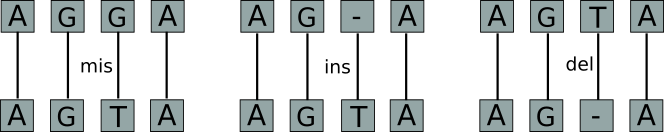
\includegraphics[scale=0.6]{Diagrams/midex.png}
\end{center}
\caption{\textit{The top character sequences are the patterns and the bottom the data. In the first example the G is simply
substituted for a T. In the second example the pattern is AGA but matches the sub-sequence AGTA in data by insertion of a
T. In the third example the pattern AGTA matches the data AGA by deleting the T.}}
\end{figure}
%\begin{figure}[H]
%\begin{tikzpicture}
%[->,node distance=1.5cm and 0.2cm, main node/.style={rectangle,fill=blue!8,draw,font=\sffamily\bfseries}] 
%\node[main node](1)    {A};
%\node[main node](2) [right= of 1] {G};
%\node[main node](3) [right= of 2] {G};
%\node[main node](4) [right= of 3] {A};
%
%\node[main node](5) [below= of 1] {A};
%\node[main node](6) [below= of 2] {G};
%\node[main node](7) [below= of 3] {T};
%\node[main node](8) [below= of 4] {A};
%
%\node[main node](9) [right= of 4, xshift=+2cm] {A};
%\node[main node](10) [right= of 9] {G};
%\node[main node](11) [right= of 10] {--};
%\node[main node](12) [right= of 11] {A};
%
%\node[main node](13) [right= of 8, xshift=+2cm] {A};
%\node[main node](14) [right= of 13] {G};
%\node[main node](15) [right= of 14] {T};
%\node[main node](16) [right= of 15] {A};
%
%\node[main node](17) [right= of 12, xshift=+2cm] {A};
%\node[main node](18) [right= of 17] {G};
%\node[main node](19) [right= of 18] {T};
%\node[main node](20) [right= of 19] {A};
%
%\node[main node](21) [right= of 16, xshift=+2cm] {A};
%\node[main node](22) [right= of 21] {G};
%\node[main node](23) [right= of 22] {--};
%\node[main node](24) [right= of 23] {A};
%
%\path[every node/.style={font=\sffamily\small}]
%(3) edge node [left] {mismatch} (7)
%(11) edge node [left] {insertion} (15)
%(19) edge node [left] {deletion} (23);
%\end{tikzpicture}
%\caption{\textit{The top character sequences are the patterns and the bottom the data. In the first example the G is simply
%substituted for a T. In the second example the pattern is AGA but matches the sub-sequence AGTA in data by insertion of a
%T. In the third example the pattern AGTA matches the data AGA by deleting the T.}}
%\end{figure}
\subsection{Backtracking}
Finding a match between data and a \pu with allowed edits often requires trying 
different combinations of uses of the edits, and \emph{backtracking} is a sort of algorithm that offers this functionality.
Backtracking is the foundation for string search in \scm and in our re-implementation. \\ \\
An implementation similar to
\scm that allows complex patterns to be defined by separable \pus would often require more than just finding \textit{one}
match for a particular \pu with allowed single-character edits. One possible combination of the single-character
edits used to find a match for one particular \pu may result in a valid match of the whole pattern, 
where other combinations that makes a particular \pu match, may prevent a whole match from being possible.
It is therefore necessary for our particular \pu to be able to find more than one way to make a valid match (if these are
possible). Consider the example in Figure 2 where the pattern is \\ \\
\texttt{CT\; AGCA[2,1,0]\; CG}, i.e. 2 mismatches and
one deletion allowed for the second PU, and the data is \\ \\
"CTAGACGT"
\begin{figure}[H]
\begin{center}
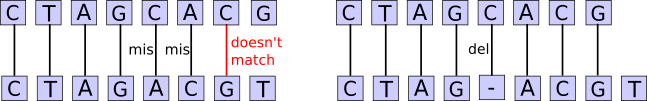
\includegraphics[scale=0.8]{Diagrams/back.png}
\end{center}
\caption{\textit{In the leftmost example the} \pu \texttt{AGCA} \textit{chooses to use 2 mismatches to match the 
data sub-sequence} "AGAC" \textit{and then move on the next} \pup \textit{The next} \pu
\textit{would then have to match it's letters} \texttt{CG} \textit{with the data sub-sequence} "GT"
\textit{which it can't do without edits. The overall algorithm would have to backtrack the the second
} \pu \textit{to try another possible match (if any) to see if that would make a difference. The rightmost example
shows how using a deletion to delete the C in} \texttt{AGCA} \textit{would match data} "AGA" \textit{and
when moving forward to the next} \pu \texttt{CG} \textit{will match} \texttt{CG}}
\end{figure}
\noindent There are two different ways for a \pu to have multiple different matches with a sub-sequence in data. 
Either it's an exact or reference \pu with allowed mismatches,
insertions and deletions, or it is a range \pup
Whenever backtracking to one of these, another of the possibilities will be chosen and the algorithm continues to the
subsequent \pu again. The amount of checks that the algorithm would need to perform in order to try out
all possibilities grows in an exponential fashion with the number of \pus and the number of different matches each
\pu has. One could visualize this as a search tree structure, 
where each horizontal level of the tree represents a single \pup The different nodes in each horizontal level
then each represent a different way of matching the overall pattern with data until reaching this \pup 
The edges from parent node to children nodes would then represent the different possibilities of matching the given
\pu with the data.
The nodes would have varying number of branches since \pus have a varying number of ways to match with a give data sub-sequence.
The height of the tree would also vary because which branch is chosen may affect what 
possibilities the subsequent \pu has, and the final \pu may not be reached with every combination. \\
Consider the example in Figure 3 where the pattern is \\ \\
\texttt{AGC[1,1,0]\; TCT[0,1,0]\; TG $<$more} \texttt{PUnits}$>$ and the data \\ \\
"ACCTCTTG$<$more data$>$" \\ \\
Using a deletion to match \texttt{AGC} with "ACC" turns out to be the "wrong" way to go down the tree. This path only
goes down 2 levels in the tree before it becomes impossible to go further. Choosing a mismatch to match \texttt{AGC} with "ACC"
and then matching \texttt{TG} with "TG" without using edits lets us further down the tree (and possibly to the last PU). \\
\begin{figure}[H]
\begin{center}
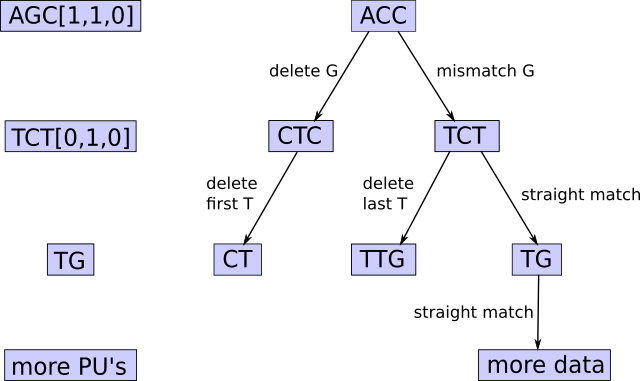
\includegraphics[scale=0.65]{Diagrams/tree.png}
\end{center}
\caption{\textit{The rectangles on the left show the \pus and each horizontal level of the tree represents the \pu 
which is horizontally aligned with it. The letter combination inside each node in the tree shows the part of the data sequence
that the given \pu tries to match with. The text attached to each edge says what choice of use of edits was made 
in order to match.}}
\end{figure}
\noindent It may be that not every path down the tree reaches the last \pu so even though the number of combinations that 
should possibly be tried grows exponentially, it can often times be determined before
reaching the bottom of the tree whether that particular way down is possible or not and if not, the combination does
not have to be checked all the way to the end. \\ \\
The worst case running time would still be exponential since it is possible for a pattern that no possible choice of match
for any \pu would prevent any of the following choices, i.e. the tree would have a homogeneous height, and
all the nodes would have their respective maximum amount of child nodes. \\ \\
Many of the sub-paths in a tree like this may yield the same result on the sub-path's end node, i.e. at a horizontal
level in the tree there may be several identical nodes, and the children of these identical nodes will of course be
identical as well, so when counting towards the number of \emph{different} overall matches, only one of these identical
branches should be considered. \\ \\
Let us define the function $children(\pu)$ to take the a \pu as input and return the amount of possible matches with	
\textit{different lengths} on any data, that the input \pu can have.
In case of mismatches insertions and deletions, the number of characters a match can differ is determined by 
the sum of the insertions (use of these makes the match longer)
and the deletions (use of these makes the match shorter). The last option is using none of the insertions or deletions which
result in yet another match length. \\ \\
If it's a range \pu then the number of different lengths are given by the size of the interval. \\ \\
$children(PU)=
\left\{
\begin{array}{ll}
(PU.max - PU.min) + 1 & \mbox{if } PU=Range \\
PU.insertions+PU.deletions+1 & otherwise 
\end{array}
\right.$
 \\ \\
Let $p$ be a pattern and $p[i]$ be the i'th \pu in $p$, and let $n$ be the number of \pus in $p$,
then the amount of combinations of the different matches of the \pus would be $comb(p)$ \\ \\
$comb(p,n)=\mathlarger{\mathlarger{\prod}_{i=1}^{n}\;children(p[i])}$ \\ \\
Consider the pattern \texttt{AGGT[0,1,1]\; 4...5\; TTCTAA[0,2,1]} called $p1$: \\ \\
$comb(p1,n)=\mathlarger{\mathlarger{\prod}_{i=1}^{3}\;children(p1[i])}= \\ \\
children(\texttt{AGGT[0,1,1]})\;\cdot \;children(\texttt{4...5})\;\cdot \;children(\texttt{TTCTAA[0,2,1]})=
3\cdot 2\cdot 4=24$ \\ \\
A total of 24 leaves on the tree. \\
As mentioned this is the maximum amount of checks that would need to be performed in order to determine if there is a 
possible match at a specific starting position in the data. Even if a tree has a homogeneous 
height, the probability of checking the correct branch lastly is low.
The average actual running time of an algorithm that uses these principles would therefore be significantly better, 
but worst case is: \\ \\
$comb(p,n)$ given a pattern $p$ and the the number of \pus $n$ in that $p$.
\subsection{Flow of \scm}
\scm uses backtracking functionality~\cite{back} on two different levels to find the matches. 
One is the outer backtracking system that backtracks between \pus, and the other is a backtracking algorithm
for matching a single \pu if it has been allowed any mismatches, insertions or deletions. \\ \\
\scm has an outer backtracking system that controls the flow of the outer pattern match, i.e. decides whether to
move forward to the next \pu if the current \pu matched, or backtrack to the previous \pu if there was no match.
When backtracking to a previous \pu the next possibility (if any) for matching is chosen and the algorithm moves
forward again. This problem would normally be solved with recursion and/or loops, but \scm uses GOTO statements which has 
both pros and cons. \\
\begin{figure}[H]
\begin{center}
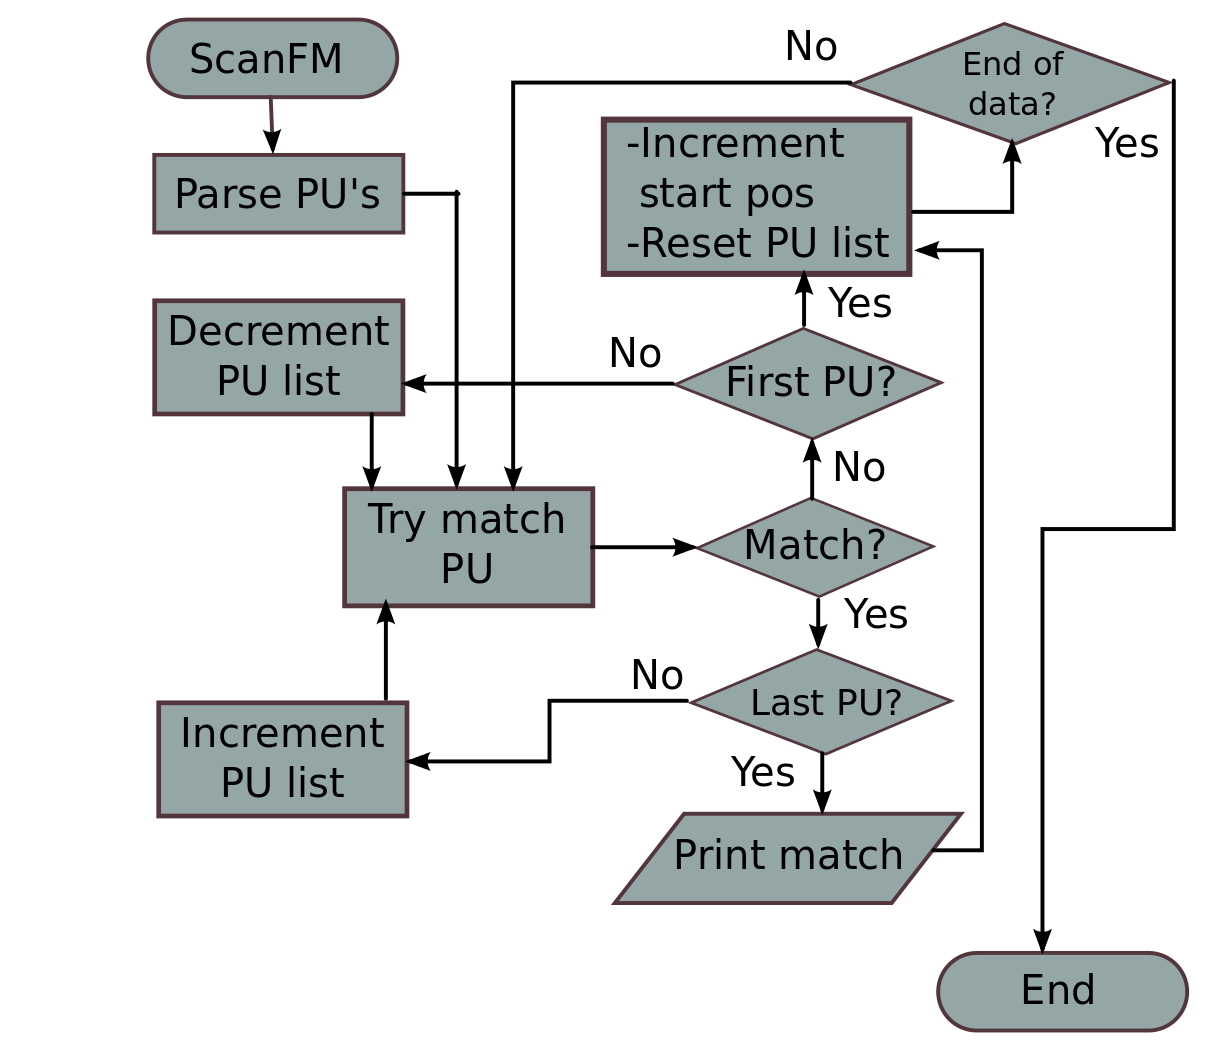
\includegraphics[scale=0.4]{Diagrams/ScanfmFlow.png}
\end{center}
\caption{\textit{Simplistic flow chart of} \scmp \textit{The blue rectangles indicate a process being executed, 
the purple diamonds indicate decisions being made, the green rounded rectangles indicate start and end of the program
and the orange parallelogram indicates output.}}
\end{figure}
\noindent The use of GOTO statements avoids some of the risks associated with the use of recursion like stack overflow. 
How deep the recursion would go would depend on the size of the pattern, and it would therefore be hard to control and
unsafe to use with respect to unwanted termination. Analyzing the possible depth of recursion and rejecting a queried search
if too deep is hardly an option, as it may be necessary to find these large patterns. \\ \\
Even though the use of GOTO statements uses a controllable fixed amount of
memory, it is not necessarily safe. The big con is the missing modularity and structure. 
It is very easy to make a mistake when creating or maintaining that sort of code
(as \scm is a great example of)
because the responsibility is not partitioned into functions or classes that can be unit-tested and proved to work.
Every variable is defined in a global scope and has to be managed as such, which is very prone to error. With every
jump back and forth between the GOTO's all variables and flags must be set just right or the behavior of the program
is undefined. 
One variable being set wrongly due to a particular input and searching in a particular part of the data may 
escalate to either deliver wrong matches or just terminate. \\ \\
Figure 4 shows the overall flow of finding patterns in \scm by backtracking back and forth between the PU's. When
a match is found it is printed to the user, the list of \pus is reset to start with the first \pu and the 
starting position in data is incremented accordingly so the search for other matches can continue. \\ \\
The other backtracking system happens internally in the pattern matching of a single \pu if that \pu has allowed
mismatches, insertions and deletions. Figuring out a way to utilize the allowed edits to possibly find a match, requires
trying out a lot of combinations so this part of the program is the most computationally heavy. 
\subsubsection{Multi-level backtracking}
Exact or reference \pus that has allowed mismatches, insertions or deletions are handled in a very specific way by \scmp
Starting from left going right in the \pu
and data, the algorithm greedily matches as many characters as possible without using allowed edits.
Every time a character doesn't match, \scm spends an edit and uses a stack structure to keep track of which
kind of edit should be tried next at this point in the sub-sequence, in case the rest of the \pu doesn't match and need to
backtrack to this spot. The different edits are tried in the following order: mismatch, deletion, insertion, i.e.
if a character doesn't match the character in data and this spot was approached from the left (not backtracking)
then a mismatch is used. When backtracking to this spot then an insertions is tried, and if that failed as well further along 
in the \pu a deletion is tried. \\ \\
By only using edits when necessary, \scm exploits the property of \emph{dominance relation}.~\cite{dom}
Dominance relation can be applied in many combinatorial problems, and allows for some of the solution
space of a problem to be dismissed as it can never be an optimal solution due to a "dominant" other part of the solution space. 
A good example is the classic knapsack problem~\cite{knap}; 
Given a set of items that each has a weight and value assigned to them,
and then a bag that can contain items up to a certain weight limit, determine how many of the different items to
include in order to maximize the total value but keeping the weight under the limit. If one of the items $I_1$ weighs
X and is worth Y, but a combination of other items (say $I_2$ and $I_3$) weighs less than X and is worth more than Y, 
then item $I_1$ can never be part of an optimal solution to this problem, since in any solution that contains $I_1$, 
one could substitute $I_1$ for $I_2$ and $I_3$ and get more value without breaking the weight limit, in which case the 
original solution containing $I_1$ was not optimal. \\ \\
The naive way of trying to fit a \pu to a sub-sequence in data using edits would be trying out every permutation of the edits
applied on the characters, even those which actually matched the data. The number of permutations would be very large,
so \scm uses dominance relation to rule out many of the permutations and speed up the search. \\
In other words, whenever \scm
encounters a character that matched the character in data, spending a mismatch, insertion or deletion is never
considered and never tried out, because the property of dominance relation promises that spending an edit
here is not necessary for finding a match. \\ \\
Figure 5 shows an example of a match between pattern and data that uses edits where it was not required,
and how one can transform this into a match that uses its first edit at the first mismatching characters.
The pattern is \texttt{ATTTTG[0,2,0]} and the data is "ATTG".
\begin{figure}
\begin{center}
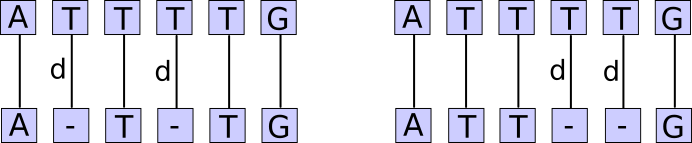
\includegraphics[scale=0.6]{Diagrams/shunt.png}
\end{center}
\caption{\textit{The leftmost example uses its two deletions where it was not necessary, and the rightmost example shows
the same match where the use of the deletions have been postponed as much as possible before being used.}}
\end{figure}
\noindent Using dominance relation \scm always finds a match for a \pu if it exists, but when used in combination
with an outer backtracking system that is not enough! \\ \\
The technique described is useful only if the goal is determining if there exist a possible match or not.
With an outer backtracking system it is often times required that several if not all possibilities are tried in
order to find the overall match. Some \pus of the overall pattern may be required to be of a specific length in order to
match the whole pattern, and the only way such a \pu can obtain the required length may very well be using unnecessary
edits. Trying to match a \pu with allowed edits, \scm will always accept the first way of matching, and even if
subsequent \pus fail and we backtrack to this \pu again, the same match with the same length will be found. \\ \\
It is therefore not guaranteed that \scm will find all the matches it's supposed to find. In fact every sub-sequence
of data that should match with the pattern, but requires for one or more of its \pus to have a length only
acquirable by using unnecessary edits, \scm will not find! \\ \\
Figure 6 shows an example of an overall pattern that will only match the data if unnecessary edits are used in a \pup
The pattern is: \texttt{AAA[0,2,0] AT} and the data is "AAAT". Only by using an unnecessary deletion in the first
\pu will the second \pu match.
\begin{figure}[H]
\begin{center}
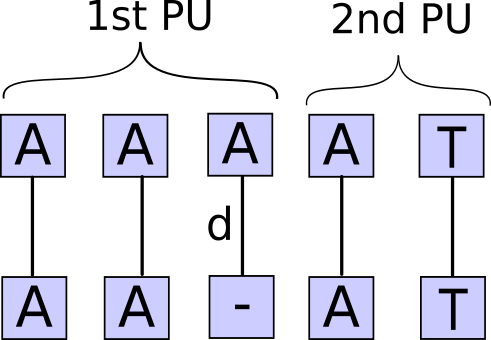
\includegraphics[scale=0.3]{Diagrams/scnfail.png}
\end{center}
\caption{\textit{The top sequences are the \pus and the bottom the data.}}
\end{figure}
\subsection{Design}
Our re-implementation of \scm called \sfm is developed in C++ rather than C, which was used to develop 
\texttt{scan\_for\_matches}. We have used C++ classes instead of C structs as the base structure for the PU's. \\ \\ 
Figure 7 shows the class structure of \texttt{scanfm}. The "Sequence" and "Range" classes inherit from the overall
class "PUnit", and the "Reference" class inherit from the "Sequence" class, since a reference \pu works exactly like a 
sequence \pu at run-time when it has collected its letter sequence from either a sequence \pu or a range \pup \\ \\
The control flow of \sfm is similar in idea to \scm but very different in implementation. While \scm uses a case/switch
and GOTO statements, \sfm uses an outer loop to call the "search" function of the \pus and then either
forward to the subsequent \pu on success or backtrack to the previous \pup \\
Passing parameters between the calls and returns of the "search" functions sets the criteria for the particular search, for
instance the search for the first \pu where the "search" function is told to search and increment data until a match is \\
found.
\subsubsection{Correctness of \sfm}
\begin{figure}[H]
\begin{center}
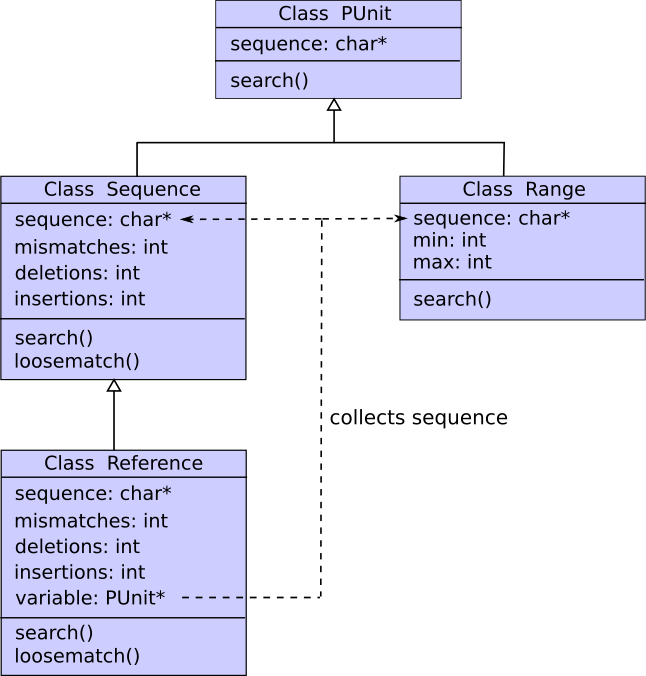
\includegraphics[scale=0.7]{Diagrams/classdia.png}
\end{center}
\caption{\textit{A simplified class diagram which only shows the most important varibles and functions.
There is one generic} \pu \textit{class called "PUnit". This class holds a lot of the common variables
and flags that are needed no matter what kind of} \pup
\textit{
Each class (except the "PUnit" class itself) defines the method "search", which searches for a match given a start position. 
The function "loosematch" is used for trying to find a match when single-character edits are allowed.}}
\end{figure}
\subsubsection{Optimizing character comparison using bitwise operations}
One of the great tricks used in \scm is the use of bitwise operations in performance critical parts of the code.
Comparing single characters is the most used operations and maximizing the speed of this particular operation 
means everything for the performance of the program. Figure 8 shows how \scm transforms every normal C character into
a custom 4-bit code. These 4 bits are used to represent each of the four letters (A,T,C and G) by having a 1 in one of
the slots and 0 in the other three. The letter G for example is represented as 0100. All possible permutations of 
combining these letters are also represented by a permutation of the bit field, e.g.\ the letter V is written in a \pu 
represents either A,C or G and therefore has the bit field 0111 since A is 0001 and C is 0010. \\
Prior to searching, the data input is of course also transformed to 4-bit representations.
When comparing two characters \scm uses the bitwise AND operator and if the result is not 0000 the characters matches. \\ \\
\scm actually stores 4 more bits (left of our 4-bit field) The complementary letter of the letter represented in the rightmost
bit field is stored in the leftmost bit field, e.g. G would look like 0010 0100 although only on of the 4-bit fields would
be used in a comparison. This leftmost bit field is used when comparing a complementary reference \pu instead
of transforming back and forth between the letters every time a complementary \pu is encountered. \\ \\
We are using this exact technique in \sfm to achieve the same optimal way of comparing characters.
\begin{figure}
\begin{center}
\begin{lstlisting}
int build_conversion_tables()
{
    int the_char;

    for (the_char=0; the_char < 256; the_char++) {
        switch(tolower(the_char)) {
          case 'a': \pu_to_code[the_char] = A_BIT; break;
          case 'c': \pu_to_code[the_char] = C_BIT; break;
          case 'g': \pu_to_code[the_char] = G_BIT; break;
          case 't': \pu_to_code[the_char] = T_BIT; break;
          case 'u': \pu_to_code[the_char] = T_BIT; break;
          case 'm': \pu_to_code[the_char] = (A_BIT | C_BIT); break;
          case 'r': \pu_to_code[the_char] = (A_BIT | G_BIT); break;
          case 'w': \pu_to_code[the_char] = (A_BIT | T_BIT); break;
          case 's': \pu_to_code[the_char] = (C_BIT | G_BIT); break;
          case 'y': \pu_to_code[the_char] = (C_BIT | T_BIT); break;
          case 'k': \pu_to_code[the_char] = (G_BIT | T_BIT); break;
          case 'b': \pu_to_code[the_char] = (C_BIT | G_BIT | T_BIT); break;
          case 'd': \pu_to_code[the_char] = (A_BIT | G_BIT | T_BIT); break;
          case 'h': \pu_to_code[the_char] = (A_BIT | C_BIT | T_BIT); break;
          case 'v': \pu_to_code[the_char] = (A_BIT | C_BIT | G_BIT); break;
          case 'n': \pu_to_code[the_char] = (A_BIT | C_BIT | G_BIT | T_BIT); break;
          default:
            \pu_to_code[the_char] = 0;
            break;
        }
        if (\pu_to_code[the_char] & A_BIT)
            \pu_to_code[the_char] |= T_BIT << 4;
        if (\pu_to_code[the_char] & C_BIT)
            \pu_to_code[the_char] |= G_BIT << 4;
        if (\pu_to_code[the_char] & G_BIT)
            \pu_to_code[the_char] |= C_BIT << 4;
        if (\pu_to_code[the_char] & T_BIT)
            \pu_to_code[the_char] |= A_BIT << 4;
    }
...
\end{lstlisting}
\end{center}
\caption{\textit{The function that prepares the conversion table that is used for converting both data and} PU's. 
\textit{The last 8 or so lines of code is where the left 4 bits is being set to the complementary of the letter
represented in the rightmost 4 bits.}}
\end{figure}
\subsubsection{Why not Levenshtein distance?}
The Levenshtein distance between two strings is defined as \textit{the minimum amount of single-character edits required
to change on string into the other.}~\cite{leve} \\ \\
Calculating the Levenshtein distance can be done quite efficiently, at least faster than our implementation calculates
every possible match given the specific three amounts of single-character edits. One could think that a faster 
implementation would be just summing
the number of allowed mismatches, insertions and deletions, calculating the Levenshtein distance between data sub-sequence
and \pu and then comparing to see if the allowed sum was exceeded. This would not be correct since
calculating the Levenshtein distance does not include requirements for the distribution of the different 
single-character edits, it just finds the minimum \textit{sum} of them. \\ \\
If the task at hand is to determine whether two strings are within a maximum allowed Levenshtein distance of each other,
then simply calculating the Levenshtein distance would be enough. 
If however the task is to determine whether one string can be changed into another string with a maximum amount of $X$  mismatches, $Y$ insertions and $Z$ deletions one can \textit{not} simply calculate the Levenshtein distance of the two
strings and compare the number to the sum of the different edits ($X+Y+Z$) since the Levenshtein distance may not live
up to the additional requirements of a maximum of either of the different edits. An example of this is shown in Figure 9. \\
\begin{figure}[H]
\begin{center}
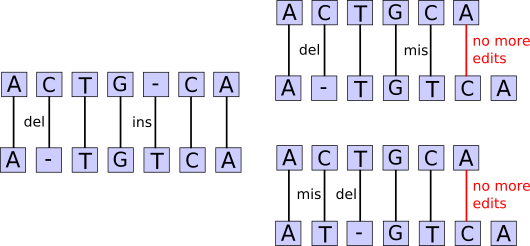
\includegraphics[scale=0.8]{Diagrams/leven.png}
\end{center}
\caption{\textit{The Levenshtein distance between the pattern ACTGCA and the data ATGTCA is 2 
(1 deletion, 1 insertion) as the leftmost example shows. If the pattern is allowed 1 deletion and 1 mismatch, then
the two strings can not match, as the rightmost examples show, even though this also would be a sum of 2 edits.}}
\end{figure}
\subsubsection{Optimizing order of \pu matching}
A possible optimization that \scm does \textit{not} exploit, is choosing an order of \pus to be searched for.
Some \pus are more exclusive and rare to find in data than others. Specifically the sequence \pu with the most
letters is the \pu that is probably found least times in a big data file. If starting the search by
identifying this rarest \pu the search would save a lot of instructions. \scm starts every search with the 
first \pu in the pattern, and it is therefore often guaranteed to run slower than if it used the other approach.
As Figure 10 shows, this optimization presents a potential huge increase in running time of the program. \newpage
\begin{figure}[H]
\begin{center}
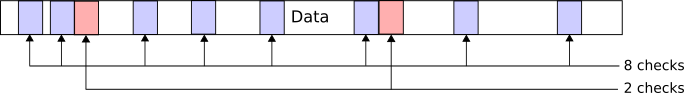
\includegraphics[scale=0.8]{Diagrams/opti.png}
\end{center}
\caption{\textit{A pattern that consists of two} \pus \textit{where the second (say} \texttt{CTCGAATAG[1,0,0]}
\textit{) is more rare in the data than the first} \pu \textit{(say(}\texttt{GGT}\textit{). Searching for the 
second} \pu \textit{first needs three checks (with three additional check afterwards to verify the whole pattern)
while choosing the look for the first} \pu \textit{needs 6 checks (with 6 following checks to verify whole pattern).}}
\end{figure}
\section{Correctness Test}
In order to show that each \pu works and returns the correct and expected results, they need to be tested individually and in specific combinations. This is done with the use of equivalence classes, this means proving that the edge scenarios of each 
\pu and average scenarios returns the expected result, and by doing so providing a by statistically solid foundation that 
the \pu is correct. 
\subsection{Individual \pu}
\subsubsection{Sequence}
To create exhaustive equivalence classes for the \pu sequence, there are multiple scenarios needed to be proven.
A sequence can be exact by having no mismatches, insertions or deletions, it can be loose fitting by having 
mismatches, insertions and deletions or it can be combined with ambiguous bases.
The equivalence class for the exact sequence, needs a test at 0, the smallest possible length and one with multiple
bases:
\begin{table}[H]
\begin{tabular}{p{4cm}|p{3.6cm}|p{2.5cm}|p{2.2cm}|p{2.2cm}}
Case 			& Pattern & Data & Expected Result & Result \\ \hline
Empty string		& " " & ACGTNNN & suiting error message & No matches \\ \hline
Single base 		& "A" & ANNN & Match at 1 & Match at 1\\ \hline
Multiple bases	& "ACCGT" & ACCGTNNN & Match at 1 & Match at 1 \\ \hline
\end{tabular}
\end{table}

The equivalence class for the loose sequence, with mismatches, insertions and deletions has more edge scenarios.
A case with 0 is needed, but in this class there are multiple scenarios for the smallest possible amount of 
mismatches, insertions and deletions, since these are not equivalent they are all needed to be tested. Also the 
combinations of the mismatches, insertions and deletions needs to be tested with both the smallest possible
scenarios and average cases. Finally the scenarios with all of the possible mismatches, insertions and deletions 
being used needs to be tested with both the smallest scenario and a average case.
With deletions and mismatches there are also the scenario where they exceed the pattern length. This also needs to 
be tested.
\begin{table}[H]
\begin{tabular}{p{4cm}|p{3.6cm}|p{2.5cm}|p{2.2cm}|p{2.2cm}}
Case 			& Pattern & Data & Expected Result & Result \\ \hline
MID 0			& "ACGT[0,0,0]" & ACGTNNN & Match at 1 & \\ \hline
MID 1 miss		& "ACC[1,0,0]" & ACGNNN & Match at 1 & Match at 1\\ \hline
MID 1 del		& "ATG[0,1,0]" & AGNNN & Match at 1 & Match at 1 \\ \hline
MID 1 ins		& "ACC[0,0,1]" & ATCCNNN & Match at 1 & Match at 1\\ \hline
MID 2 			& "AGGT[1,1,0]" & ACTNNN & Match at 1 & \\ \hline
MID 2			& "ACGT[1,0,1]" & AGTGTNNN & Match at 1 & \\ \hline
MID 2 			& "ATTGT[0,1,1]" & ATCGTNNN & Match at 1 & \\ \hline
MID 3			& "AACGT[1,1,1]" & CAGGTNNN & Match at 1 & \\ \hline
MID miss multiple & "ACCT[2,0,0]" & ATTTNNN & Match at 1 & \\ \hline
MID del multiple & "AGTTT[0,2,0]" & AGTNNN & Match at 1 & \\ \hline
MID ins multiple & "ACGT[0,0,2]" & ACTTGTNNN & Match at 1 & \\ \hline 
MID multiple		& "ACTTT[1,2,0]" & GCTNNN & Match at 1 & Match at 1\\ \hline
MID multiple		& "TCGAT[3,0,2]" & CGCTTATNNN & Match at 1 & \\ \hline
MID multiple		& "TCGGT[0,2,3]" & GGGGGTNNN & Match at 1 & \\ \hline
MID all			& "ATTCCCTT[2,2,1]" & TTCCGTAN NN & Match at 1 & Match at 1\\ \hline
MID more del		& "ATTC[0,6,0]" & CCCCCCNNN & A unknown number of matches not equal to 0
\footnote{Since the code does not specify a order of used deletions, the 
length of the match can be everywhere from 0 to 4, making it hard to predict a result. 
This does not mean that different results can't all be correct. } & \\ \hline
MID more mis		& "ATTCG[8,0,0]" & GGGGTNNN & Match at 1 & \\ \hline
\end{tabular}
\end{table}



In order to create a equivalence class for ambiguous bases in a exact sequence \pu, the same
scenarios as a exact sequence is needed with the addition that all ambiguous bases needs to be
shown to work individually. 
\begin{table}[H]
\begin{tabular}{p{4cm}|p{3.6cm}|p{2.5cm}|p{2.2cm}|p{2.2cm}}
Case 			& Pattern & Data & Expected Result & Result \\ \hline
Single ambiguous base & "R"(R is A or G) & ATTGNNN & Match at 1 and 4 & Match at 1 and 4 \\ \hline
Ambiguous bases	& "RRGGWW" & AAGGTANN N & Match at 1 & Match at 1 \\ \hline
All ambiguous bases & "UMMRRWWS SYYKKBBB DDDHHHVV VNNNN" & TACAGATC GCTGTCGT AGTACTAC GACTGNNN & Match at 1 & \\ \hline
\end{tabular}
\end{table}

In order to make sure that ambiguous bases work correctly with the defined bases, a equivalence class is needed
to show that the smallest mixed scenario and a average scenario works correctly.
\begin{table}[H]
\begin{tabular}{p{4cm}|p{3.6cm}|p{2.5cm}|p{2.2cm}|p{2.2cm}}
Case 			& Pattern & Data & Expected Result & Result \\ \hline
Smallest mix		& "AM" & ACAA & Match at 1 and 3 & \\ \hline
Average mix		& "TTATMTNYY" & TTATATGTC & Match at 1 & 
\end{tabular}
\end{table}


\subsubsection{Range}
Range by itself does not make room for a large difference in possibilities, in order to create a 
equivalence class only a few scenarios are needed, the smallest possible cases, a 0 case and a average case.
\begin{table}[H]
\begin{tabular}{p{4cm}|p{3cm}|p{2.5cm}|p{2.5cm}|p{2.5cm}}
Case 			& Pattern & Data & Expected Result & Result \\ \hline
Range from 0...0	& "0...0" & ACCNNN & Match at 1, 2 and 3 & Never ending loop \\ \hline
Smallest range 	& "0...1" & ACCNNN & Match at 1, 2 and 3 & Never ending loop \\ \hline
Smallest range without 0 & "1...1" & AGTNNN & Match at 1, 2, 3, 4, 5 and 6 & \\ \hline
Standard case	& "4...9" & AAAAAAAA AANNN & Match at 1 and 5 & Match at 1, 5 and 9
\end{tabular}
\end{table} 


\subsection{Multiple \pus}

\subsubsection{Reference}

Reference can't be tested and proved correct as a individual \pu since it needs to refer to another \pu
to function. 
In order to make sure the reference \pu works correctly the equivalence class needs to obtain references with and
without another \pu between the refereed \pu and the reference \pu. Both a 0, edge and average case is needed for both
scenarios.
\begin{table}[H]
\begin{tabular}{p{4cm}|p{3cm}|p{2.5cm}|p{2.5cm}|p{2.5cm}}
Case 			& Pattern & Data & Expected Result & Result \\ \hline
0 reference with 	& "p1=0...0 2...4 p1" & ACCCNNN & Match at 1 & Match at 1 \\ \hline
Smallest reference with 	& "p1=1...1 2...2 p1" & ACCANNN & Match at 1 & Match at 1 \\ \hline
Standard case with	& "p1=3...5 2...2 p1" & CCCCAACC CCNNN & Match at 1 & Match at 1\\ \hline
0 reference without	& "p1=0...0 p1" & TTGTANNN & Undefined & \\ \hline
1...1 reference without & "p1=1...1 p1" & AANNN & Match at 1 & \\ \hline
Standard case without & "p1=3...5 p1" & CACCCACC NNN & Match at 1 & Match at 1\\ \hline
\end{tabular}
\end{table}

In order to show correctness of complementary reference \pu a equivalence class needs to contain the same scenarios
as the equivalence class showing the simple reference scenario.
\begin{table}[H]
\begin{tabular}{p{4cm}|p{3cm}|p{2.5cm}|p{2.5cm}|p{2.5cm}}
Case 			& Pattern & Data & Expected Result & Result \\ \hline
Complementary 0 reference & "p1=0...0 2...2 \textapprox p1" & AAAANNN & Match at 1, 2, 3 and 4 & Match at 1 and 4\\ \hline
Complementary smallest reference & "p1=1...1 2...2 \textapprox p1" & ACCTNNN & Match at 1 & Match at 1\\ \hline
Complementary standard case & "p1=3...5 2...2 \textapprox p1" & AATTCCAA TTNNN & Match at 1 & Match at 1\\ \hline
Complementary 0 reference without & "p1=0...0 \textapprox p1" & AATNNN & Undefined behaviour & \\ \hline
Complementary smallest reference withour & "p1=1...1 \textapprox p1 & ATNNN & Match at 1 & \\ \hline 
Complementary reference after assignment & "p1=3...3 \textapprox p1" & AAATTTNN N & Match at 1 & Match at 1\\ \hline
\end{tabular}
\end{table}

Reference with mismatches, insertions and deletions equivalence class has the same basic steps as the simple reference
scenario, but because MID are all ready tested in the sequence, there is no difference in the reference and we don't
need to test with every single case of mismatches, insertions and deletions. Instead the use of the standard scenario is 
used.
\begin{table}[H]
\begin{tabular}{p{4cm}|p{3cm}|p{2.5cm}|p{2.5cm}|p{2.5cm}}
Case 			& Pattern & Data & Expected Result & Result \\ \hline
Reference MID 0 & "p1=0...0 2...2 p1[1,2,1]" & AACTGNNN & Undefined & \\ \hline
Reference MID smallest & "p1=1...1 2...3 p1[1,1,2]" & AACCNNN & Match at 1 & \\ \hline
Reference MID & "p1=3...4 2...2 p1[2,1,1]" & AAAATTCG TANNN & Match at 1 & Match at 1\\ \hline
Reference MID 0 without & "p1=0...0 p1[1,1,1]" & ACTNNN & Undefined & \\ \hline
Reference MID smallest without & "p1=1...1 p1[2,1,2]" & ACGTNNN & Match at 1 & \\ \hline
Reference MID without & "p1=3...5 p1[2,1,1]" & ACTTACNNN & Match at 1 & \\ \hline
\end{tabular}
\end{table}


Complementary reference with mismatches, insertions and deletions, in this case we make the same assumptions as above
that mismatches, insertions and deletions are proved to be correct in the individual cases from the sequence test.
Because of that we test with the same scenarios as the simple reference tests, to obtain a exhaustive equivalence class.
\begin{table}[H]
\begin{tabular}{p{4cm}|p{3cm}|p{2.5cm}|p{2.5cm}|p{2.5cm}}
Case 			& Pattern & Data & Expected Result & Result \\ \hline
Reference MID complementary 0 & "p1=0...0 2...3 \textapprox p1[1,2,1]" & ACGTGNNN & Undefined & \\ \hline
Reference MID complementary smallest & "p1=1...1 2...3 \textapprox p1[0,1,0]" & ACGGGNNN & Match at 1 & Match at 1 and 4 \\ \hline
Reference MID complementary & "p1=3...4 2...3 \textapprox p1[1,0,1]" & ACCTTGCC TNNN & Match at 1 & Match at 1 \\ \hline
Reference MID complementary 0 without & "p1=0...0 \textapprox p1[0,1,2] & ACCTNNN & Undefined & \\ \hline 
Reference MID complementary smallest without & "p1=1...1 \textapprox p1[0,0,2] & CTTCNNN & Match at 1 & \\ \hline
Reference MID complementary without & "p1=3...4 \textapprox p1[1,0,0]" & AAATACTT NNN & Match at 1 & Match at 1 \\ \hline
\end{tabular}
\end{table}


In order to make a exhaustive equivalence class for multiple \pus or multiple exhaustive equivalence classes for \pus
a great number of different combinations and scenarios would be needed. Instead the following tests performed gives a 
statistically approximation to this by looking at the scenarios that are most likely to produce false results.

\begin{table}[H]
\begin{tabular}{p{4cm}|p{3cm}|p{2.5cm}|p{2.5cm}|p{2.5cm}}
Case 			& Pattern & Data & Expected Result & Result \\ \hline
Multiple exacts 	& "ACGT TGCA" & ACGTTGCA NNN & Match at 1 & Match at 1\\ \hline
Range MID		& "4...5 TTTT[1,1,1]" & AAAAATTC GNNN & Match at 1 & Match at 1\\ \hline
Backtracking MID & "TTTT[0,1,1] TTA" & TTTTTAAN NN & Match at 1 & Match at 1\\ \hline
Multiple references & "p1=2...3 p2=2...2 p1 p2" & TTTCCTTT CCNNN & Match at 1 & Match at 1\\ \hline
Mulitple complementary reffenreces & p1=3...3 p2=2...3 2...3 \textapprox p2 \textapprox p1" & 
AAATTCCT TAATTTNN N & Match at 1 & Match at 1 \\ \hline
0 refference with bounding \pus & "AATCC p1=0...1 0...3 p1 TTG" & AATCCTTGGGGGGGNNN & Match at 1 & \\ \hline
\end{tabular}
\end{table} 
\section{Speed test}
\newpage
\printbibliography
\end{document}
